  	
  %-----------------------------------------------------------------%
  %   Architecture et explication détaillé de l'implémentation
  %-----------------------------------------------------------------%
  \chapter{Architecture du programme}
  
  Nous avons décidé de reprendre un programme existant afin d'accélérer le développement.
  Ce programme est celui de Robert Lindner, présenté dans l'état de l'art (cf: ~\nameref{sec:lard-projets}).
  
  \section{Lancement du programme}
  Des options de lancement ont été rajouté au programme, leurs utilisations sont disponible en annexe \ref{annexe:usage}
  

  \section{Système de rendu}
  Le programme est découpé en classes afin d'abstraire les appels à la bibliothèque OpenGL. La figure \ref{fig:uml_scene} représente le diagramme des classes qui forment l'abstraction principale du programme.
  Les classes relatives à la génération, l'affichage de la planète et l'utilisation du CDLOD sont strockés dans le dossier
  PlanetTech.
  
  \begin{figure}[!ht]
  \centering
  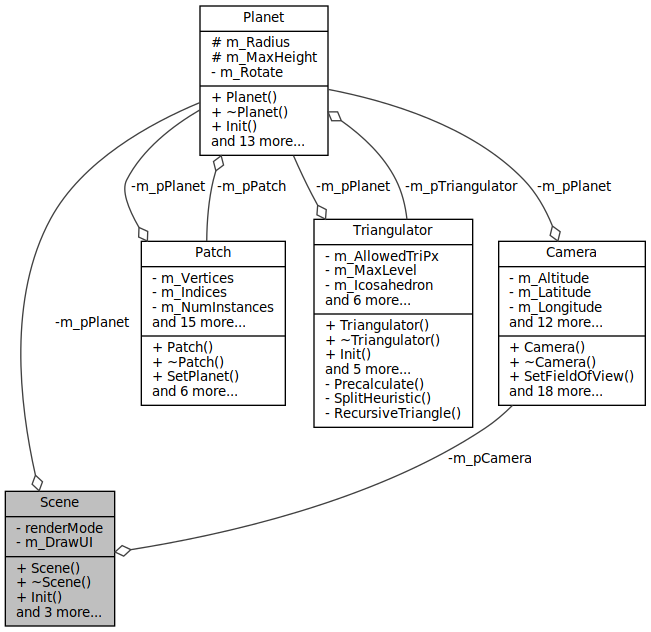
\includegraphics[width=8cm]{img/uml_scene.png}
  \caption{Diagramme des classes principales}
  \label{fig:uml_scene}
  \end{figure}

  La classe Scene est la classe centrale du programme, elle permet
  d'initialiser et de créer la planète. Scene gère les paramètres
  principaux du programme à travers les entrées clavier d'InputManager.
  Ces paramètres sont le nombre de niveaux de détail, le mode d'affichage
  (texture + maillage, maillage uniquement, texture uniquement). Scene
  gère aussi l'affichage des informations comme le compteur d'images par
  seconde ou le nombre de sommets actuellement affichés.\\
  
  \begin{figure}[!ht]
  \centering
  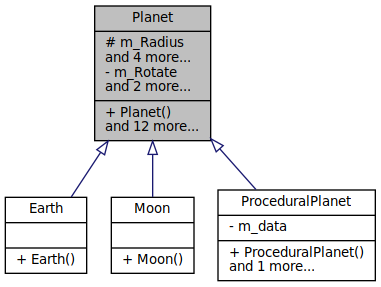
\includegraphics[width=5cm]{img/planet_inh.png}
  \caption{Diagramme d'héritage de Planet}
  \label{fig:inh_planet}
  \end{figure}

  La classe Planet représente la sphère à afficher. Ses classes filles
  (voir figure \ref{fig:inh_planet} spécialisent le type de planète
  à afficher, ce sont elles qui définissent la taille de la sphère,
  sa texture et sa carte de hauteur.\\

  \newpage
  \newpage
\section{Heightmap}
  
  Le programme utilise un \emph{quadtree} pour générer les différents niveaux de détail. 
  Ensuite une nouvelle hauteur est appliquée à ce point pour le déplacer. 
  Cependant, le \emph{quadtree} ne stocke pas la hauteur du sommet. Cette dernière
  est enregistrée dans une texture 2d qui est envoyée à la carte graphique. 
  Chaque pixel de la texture représente donc une valeur codée sur un nombre flottant entre 0 et 1.
  La texture récupérée par la carte graphique, est plaquée sur le maillage de la sphère et la hauteur du sommet
  est déduite de l'interpolation des texels\footnote{Un texel est une unité d'une texture, il est l'homologue du pixel sur une image.} de la texture sur le maillage.
    %définir texel
  %définir interpolation ?
  
  \section{Triangulator}
  La classe Triangulator permet de générer le \emph{quadtree} utilisé pour le système de niveau de détail.
  Un objet Frustum est utilisé pour décider si un triangle de l'arbre est ou non dans le cône 
  de vision de la caméra. Le diagramme de classes présenté en figure \ref{fig:plan} présente la classe
  Triangulator. Les différents composants seront analysés plus loin dans le chapitre implémentation.
  
  \section{Patch}
  La classe Patch récupère les triangles envoyés par Triangulator, et les subdivisent (beaucoup) tout en appliquant l'algorithme de morphing. La subdivision n'est calculée qu'une seule fois à l'initialisation, tous les triangles sont ensuite subdivisés de la même façon. Le morphing permet non seulement d'adoucir les différences entre les niveaux de détails et mais aussi et surtout d'éliminer les trous.
  
  
  \begin{figure}
  \centering
  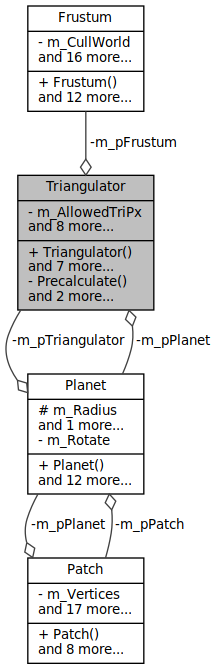
\includegraphics[width=5cm]{img/tri_class2.png}
  \caption{Diagramme de classe de Triangulator}
  \label{fig:plan}
  \end{figure}
  
  \section{Frustum}
  La classe Frustum permet de faire la différence entre un triangle dans le champ, un triangle partiellement dans le champ, et un triangle hors champ. Le Frustum est utilisé par la classe Triangulator lors de la construction du maillage.\\
  
  Les triangles hors du champ de la caméra ne sont pas affiché à l'écran, il n'est donc pas nécessaire de les envoyer à OpenGL pour qu'ils soient dessinés. 
  
  Cette classe a donc pour but d'éliminer les triangles qui ne sont pas visibles. Cette opération appelée \textit{culling} accélère la génération en supprimant des noeuds de récursion, diminue la taille de transfère entre CPU/GPU, et diminue le nombre de triangles à dessiner dans la carte graphique.
  
  \section{Gestion des paramètres utilisateur}
  
  À été rajouté au sein du programme un système permettant à l'utilisateur de renseigner diverses paramètre au lancement du programme. Les paramètres sont récupéré sous forme d'un tableau de chaînes de de caractères.\\
  Ils sont ensuite traités grâce à la classe \textit{ArgvParser} qui est expliquée plus en détails dans la partie (\ref{sec:argvparser}). Les différents paramètres sont établies sous la forme d'un usage (\ref{annexe:usage}).
  
 \newpage %pour placer les images correctement
 